\documentclass{standalone}
\usepackage{tikz}
\usetikzlibrary{shapes,arrows.meta}
\begin{document}
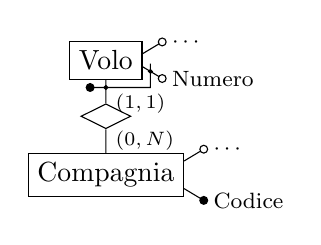
\begin{tikzpicture}
    \draw

    %%* Attributi:
    %%  node[draw, circle, inner sep=1pt, fill=black]{}node[right]{\footnotesize A}
    %%? Distanza orizzontale: E -(0.25,0.x)- A
    %%? Distanza verticale: E -(0,x * 0.22)- A

    %%* Cardinalità:
    %%  node[below right]{\scriptsize $(0,N)$}
    %%  node[above right]{\scriptsize $(0,N)$}
    %%  node[midway, above]{\scriptsize $(0,N)$}

    %%* Relazione:
    %%  node[draw, diamond, shape aspect=2, inner sep=3pt, anchor=90](r1){}
    %%  node[draw, diamond, shape aspect=2, inner sep=0.2pt, anchor=180](r2){R2}

    %%* Entità:
    %%  node[draw, rectangle, anchor=90](e1){}
    %%? Distanza verticale: E -(0.3)- R -(0.3) E
    %%? Distanza orizzontale: E -(0.75)- R -(0.75)- E

    %%* Conto Corrente
    (0,0)node[draw, rectangle, anchor=90, align=center](cc){Volo}
    (cc.270)--++(0,-0.1)node[draw, circle, inner sep=0.5pt, fill=black](a){}--++(0,-0.2)node[right]{\scriptsize $(1,1)$}node[draw, diamond, shape aspect=2, inner sep=3pt, anchor=90](r2){}
    (cc.350)--++(0.1,-0.06)node[draw, circle, inner sep=0.5pt, fill=black](b){}--++(0.15,-0.09)node[draw, circle, inner sep=1pt, fill=white]{}node[right]{\footnotesize Numero}
    (cc.10)--++(0.25,0.15)node[draw, circle, inner sep=1pt, fill=white]{}node[right]{\footnotesize $\cdots$}
    (a)++(-0.2,0)node[draw, circle, inner sep=1pt, fill=black]{}-|(b)--++(0,0.1)

    (r2.270)--++(0,-0.3)node[midway, right]{\scriptsize $(0,N)$}node[draw, rectangle, anchor=90](bc){Compagnia}
    (bc.10)--++ (0.25,0.15) node[draw, circle, inner sep=1pt, fill=white]{}node[right]{\footnotesize $\cdots$}
    (bc.350)--++ (0.25,-0.15) node[draw, circle, inner sep=1pt, fill=black]{}node[right]{\footnotesize Codice}
    ;
\end{tikzpicture}
\end{document}